\documentclass[]{scrartcl}
	
%opening
\title{Orbital Gravity Simulation}
\subtitle{An implementation of newtonian mechanics in Scala and OpenGL}
\author{Freddie Poser}
\date{2016}

\usepackage{hyperref} 
\usepackage{url}
\usepackage[hyphenbreaks]{breakurl}
\usepackage{xcolor}
\usepackage{listings}
\usepackage{graphicx}
\usepackage{wrapfig}
\usepackage{caption}
\usepackage[list=true]{subcaption}
\usepackage{import}
\usepackage{pgfplots}
\usepackage[section]{placeins}

\usepackage{tikz}
\usetikzlibrary{shapes,arrows}

\graphicspath{ {img/} }
\lstset{
	basicstyle=\small\ttfamily,
	numbers=left,
	breaklines=true,
	postbreak=\raisebox{0ex}[0ex][0ex]{\ensuremath{\color{red}\hookrightarrow\space}},
	keywordstyle=\color{orange},
	stringstyle=\color{darkgreen},
	commentstyle=\color{gray},
	morecomment=[l][\color{magenta}]{\#}
}

\lstdefinelanguage{Scala}{	
	morekeywords={abstract,case,catch,class,def,
		do,else,extends,false,final,finally,
		for,if,implicit,import,match,mixin,
%		new,null,object,override,package, 
		private,protected,requires,return,sealed,
		super,this,trait,true,try,
		type,val,var,while,with,yield},
	sensitive,
	morecomment=[l]//,
	morecomment=[n]{/*}{*/},
	morestring=[b]",
	morestring=[b]',
	morestring=[b]""",
}
\lstset{language=Scala}
\begin{document}

\maketitle

\begin{abstract}
An implementation of Newtonian mechanics designed to simulate gravity and interactions between particles in two dimensions.
\end{abstract}

\tableofcontents
\listoffigures
\newpage

\section{Plan}
	The plan for this project is to simulate the motion of round particles in two dimensions. The particles will exert Newtonian gravity on each other and will be able to collide. This will all be implemented using Newtonian mechanics, namely Newton's second law and the kinematic laws of motion.
	
	For the motion I will assume that acceleration is constant for 1 second and so the simulation will update in steps, each representing 1s. It may be possible in the future to decrease this for more accurate simulations (or increase it for faster ones).
	
	I am going to build this in with Scala, a JVM programming language. The advantage of Scala is that it is multi-paradigm, allowing me to use OOP and functional programming concepts. For the graphics I will use an OpenGL wrapper library called LWJGL\footnote{\url{https://www.lwjgl.org/}}.
	
	Using this will allow me to watch the simulation in real-time rather than look at the data it outputs after the fact. I may implement a way of getting the raw data out of the simulation as well so that I can simulate real situations with greater ease.
	
	Below is an overview of the features that I implemented in the program. They are covered in the order that I implemented them.
\newpage
\section{Setup}
	
	\sloppy
	All of the source code is available at \burl{https://github.com/vogon101/NewtonianMechanics}
	
	Below is a list of a few of the core classes in the simulation
	
	\subsection{Universe}
		\fussy	
		The Universe class manages the overall simulation. The key part of Universe is its list of all the particles in existence. The Universe also contains the GraphicsManager which controls all of the rendering and adds a layer of abstraction between the simulation and the OpenGL bindings. 
		
	\subsection{Particle}
		
		The Particle class represents every single object in the system. The particles all have a ParticleType which defines their intrinsic properties: radius, mass, colour as well as a position vector. Each particle is able to render itself which involves drawing the appropriate circle at its location, the path that it has been on and all of the forces acting on it.
		\linebreak\linebreak
		The key physics is contained in the methods interact(that: Particle) and runTick():
		
		\subparagraph{interact}
		
			Interact is called by the universe class before every tick is run. For every unique pair of particles in system interact is called once. It takes in the particle to interact with and returns a list of forces generated by the interaction.
			
			These forces are then taken by the universe class and applied to their target particles, storing them up for the next time runTick is called.
		
		\subparagraph{runTick}
			
			RunTick is called on every particle each time the simulation updates after all of the interactions are computed. It returns no value but instead computes the effects of the forces and updates the particles position and velocity accordingly.
			
			The effective input to runTick is a list of forces and it then performs the following calculations (t = length of tick in this case):
			
			\begin{figure}
				\begin{equation}
					\vec{F_{R}} = \vec{F_{1}} + \vec{F_{2}} ... \vec{F_{n}}
				\end{equation}
				
				\begin{equation}
					\vec{a} = \frac{\vec{F_{R}}}{m}
				\end{equation}
				
				\begin{equation}
					\vec{v} = \vec{u} + \vec{a}t
				\end{equation}
				
				\begin{equation}
					\vec{r} = \vec{r} + \vec{v}t
				\end{equation}
				\caption{Movement equations used in Particle class}
				\label{fig:movEqn}
			\end{figure}
		
			These equations are based first on Newton's second law of motion which gives that the net force on an object is equal to its mass times its acceleration ($\vec{F_{R}} = m\vec{a}$). With the acceleration I find the new velocity by multiplying it by the time it acts for and adding it to the old velocity. This model assumes constant acceleration and velocity for the duration of each tick. This means that the accuracy of the model is linked to the length of the tick, with the shorter they are, the better the simulation. The position is then found by applying the velocity in the same way.
	\newpage
	\subsection{Rendering}
		
		Rendering uses code that I originally wrote for a simple game engine (\href{https://github.com/vogon101/CottonGame}{Cotton Game})\footnote{\url{https://github.com/vogon101/CottonGame}}. This code does a number of things:
		
		\subparagraph{GraphicsManager} 
			
			The graphics manager class controls the basic screen setup and the standard OpenGL commands that need to be called to simply get rendering working.
		
		\subparagraph{Sync} 
		
			The sync class is a utility that allows the programmer to control how often a given method is run in a non-blocking fashion. In this project it is used in three places:
			
			\begin{itemize}
			\item Render Sync - locks the render loop at 60FPS
			
			\item Update Sync - allows the user to choose how fast to run the simulation
			
			\item UX Sync - separates the input polling from the update sync so that even if the game is paused the user can still control it
		\end{itemize}
		
		\subparagraph{Render} 
		
			The Render object is a static collection of utilities that make rendering easier to work with, they abstract away from the details of OpenGL so that code is cleaner and easier to debug
	
\newpage
	\section{Gravity}
	For gravity I use the Newtonian equation which provides the magnitude of the force between two bodies. I calculate this during the interact function so the force is calculated between every pair of particles in the universe.
	\begin{figure}[h]
		\begin{equation}
		F = G\frac{m_{1}m_{2}}{r^{2}}
		\end{equation}
		\caption{Newton's law of Universal Gravitation}
		\label{fig:gravEqn}
	\end{figure}\footnote{Source: \url{https://en.wikipedia.org/wiki/Newton's_law_of_universal_gravitation}}
	
	Once I have the magnitude I find its direction by finding the angle between the two position vectors and it is applied to each body.
	\begin{figure}[h]
		\centering
		\begin{lstlisting}[language=Scala]
val distance = that.position.distance(position)
val gravForce = (GRAVITATIONAL_CONSTANT * mass * that.mass) / Math.pow(distance, 2)

//Final forces from gravity
List(
  Force(that, gravForce, (this.position - that.position).theta),
  Force(this, gravForce, (that.position - this.position).theta)
)
		\end{lstlisting}
		\caption{The gravity calculations from the Particle class}
		\label{fig:gravCode}
	\end{figure}

	This creates two vector forces, one on each object which are used during the run tick phase.
	
	Whilst Newtonian gravity has been superseded by general relativity it is still a good approximation in almost all situations where great precision is not required and where the bodies move at low speeds. I have used it in this project because it is much easier to implement\footnote{\url{https://en.wikipedia.org/wiki/Newton's_law_of_universal_gravitation\#Problematic_aspects}}
	
	\begin{figure}[p]
		\centering
		\begin{subfigure}{0.9\textwidth}
			\centering
			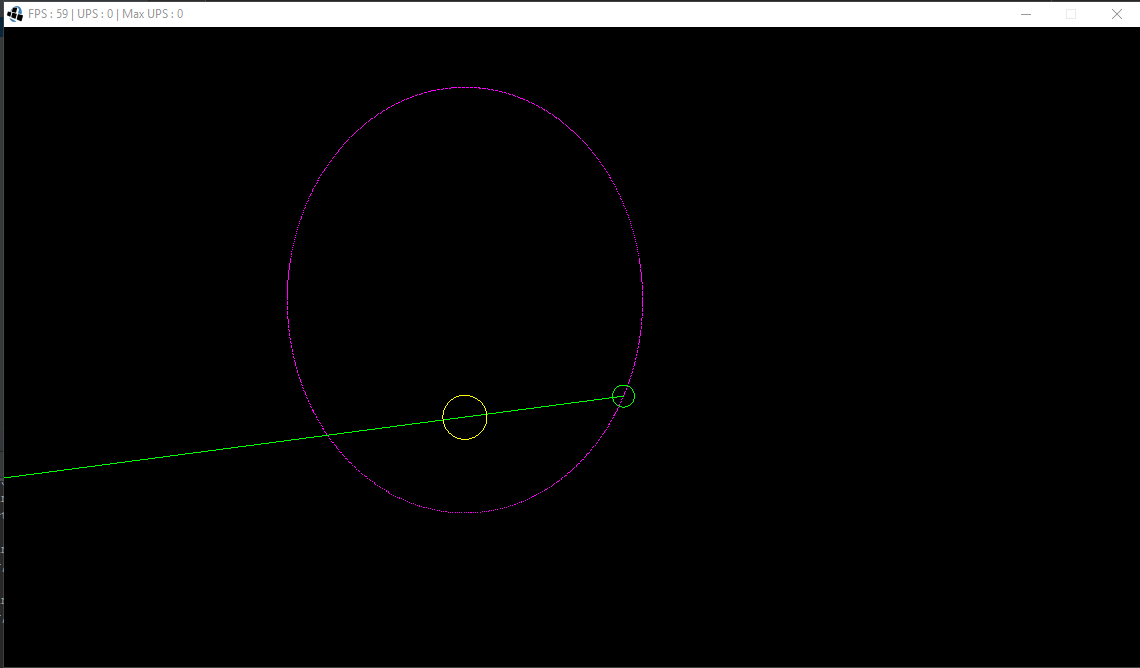
\includegraphics[width=\textwidth]{gravity1}
			\caption{One body in orbit, the orbit is perfectly stable in this case. The green line is the force on the planet.}
			\label{fig:gravExamplesSub1}
			\ref{fig:gravExamplesSub1}
		\end{subfigure}
		\begin{subfigure}{0.9\textwidth}
			\centering
			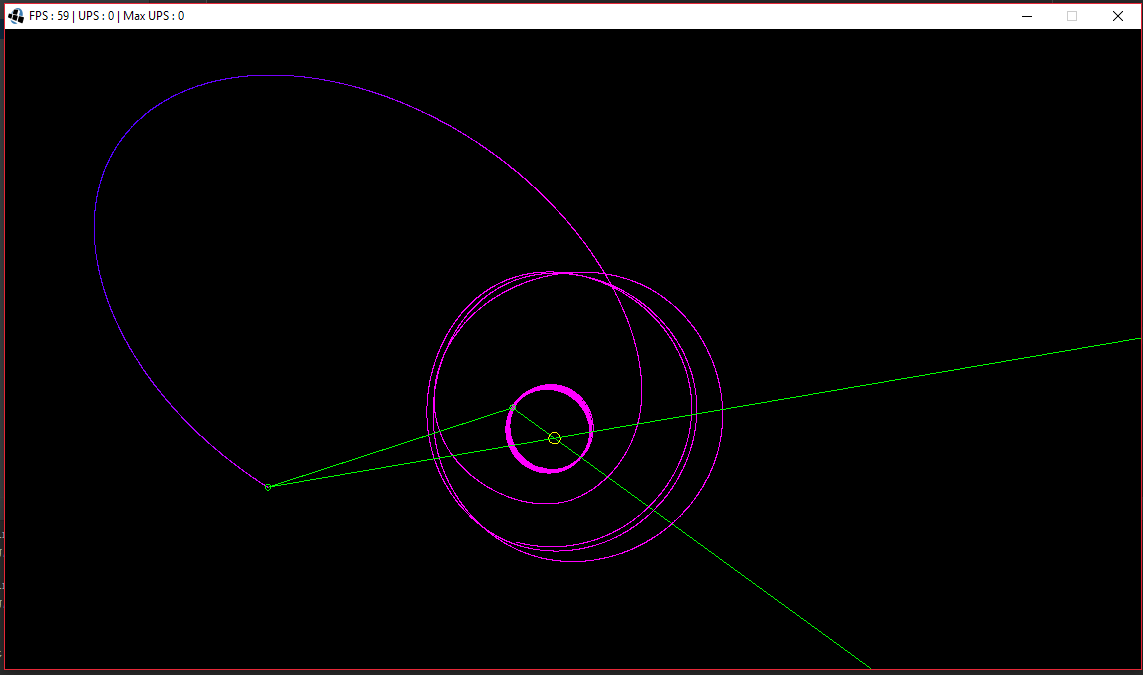
\includegraphics[width=\textwidth]{gravity2}
			\caption{Two bodies in orbit, one is on a more stable orbit whilst the outer one moves more erratically} 
			\label{fig:gravExamplesSub2}
			\ref{fig:gravExamplesSub2}
		\end{subfigure}	
		\caption{Examples of gravity with one and two bodies in orbit around a fixed star}
		\label{fig:gravExamples}
	\end{figure}
\newpage
\section{Momentum  and Collisions}
	Once I had implemented gravity I decided to add in simple 2D collisions to make the simulation slightly more realistic.
\newpage
\section{User Control}
	
	Whilst the majority of this project is the physics, I think it is important that it is possible to interact with the simulation to be able to watch it more effectively. To this end I have built a command system which allows the user to control parts of the simulation along with certain key bindings.
	
	\begin{figure}[h]
		\begin{itemize}
			\item \textbf{+}/\textbf{-} $\rightarrow$ Speed up/slow down the simulation
			\item \textbf{LSHIFT} + \textbf{+}/\textbf{-} $\rightarrow$ Zoom in/out
			\item \textbf{LEFT}/\textbf{RIGHT} $\rightarrow$ Pan around the simulation horizontally
			\item \textbf{UP}/\textbf{DOWN} $\rightarrow$ Pan around the simulation vertically
		\end{itemize}
		\caption{Key bindings for the simulation}
		\label{fig:keybindings}
	\end{figure}
	
	\begin{figure}[h]
		\begin{itemize}
			\item track $<$particle num$>$ $\rightarrow$ Track a certain particle
			\item cleartrack $\rightarrow$ Clear the tracker, allow free movement
			\item show $\rightarrow$ Print a list of particles to STD Out
			\item forces $\rightarrow$ Toggle rendering of forces
			\item col $<$on/off$>$ $\rightarrow$ Render collision forces even if force rendering disabled
			\item particle $<$particle num$>$ $\rightarrow$ Centre view on a particle
			\item pause $\rightarrow$ Pause the simulation
			\item slow $\rightarrow$ Slow down the simulation to 10 UPS
			\item 1 $\rightarrow$ Set the maximum UPS to 1 (real time)
			\item speed $<$UPS$>$ $\rightarrow$ Set the speed of the simulation (sets max UPS)
			
			
		\end{itemize}
		\caption{Commands for the simulation}
		\label{fig:commands}
	\end{figure}
	
	\begin{figure}
		\centering
		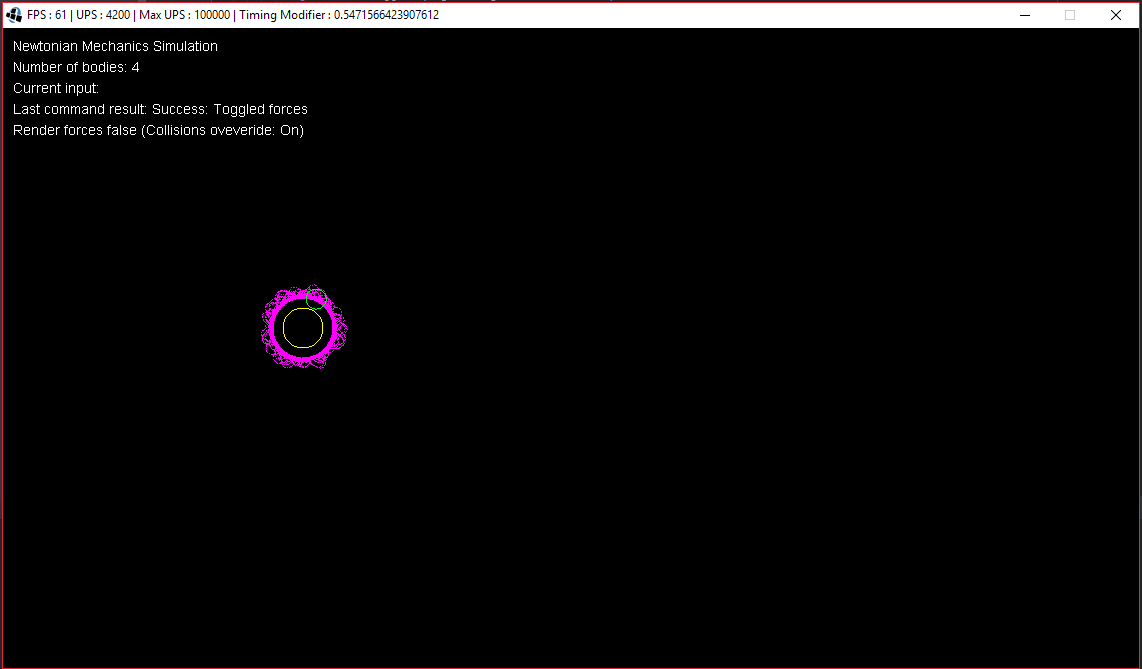
\includegraphics[width=\textwidth]{ux1}
		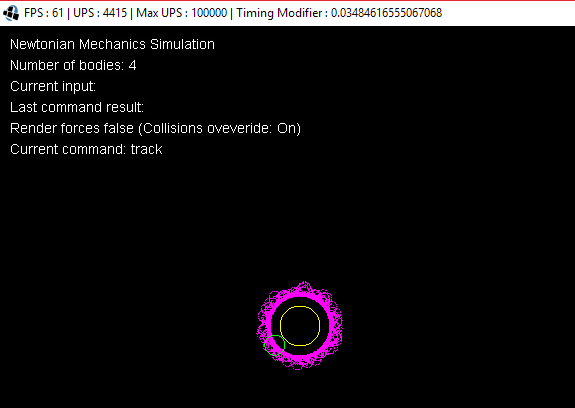
\includegraphics[width=\textwidth]{ux2}
		\caption{Information about the simulation displayed in the top left corner}
		\label{fig:uxImg1}
	\end{figure}
	
	
\newpage
\section{Diary}
	\subsection{Before Christmas}
		In the session before the Christmas break I decided that I wanted to create a simulation of Gravity. I decided on this because it seemed like a do-able project which would encompass a number of physical concepts: Newtonian gravity, constant acceleration formulae, etc as well as some interesting programming concepts.
		
	\subsection{9th Jan}
		In this session I fleshed out my idea. I decided to use OpenGL for rendering the simulation. I also implemented the core physics of the simulation: The gravity. I did this by first creating the Particle class and then implementing forces and movement. I then had every Particle exert a gravitational force on every other Particle.
	
	\subsection{16th Jan}
		Next I started work on the rendering system so that I could visualise my simulation. I used OpenGL for this. In this session I only got as far as simply rendering the circles for the particles
		
	\subsection{23rd Jan}
		By this session I had completed the core rendering with particles, forces and paths all being rendered to the screen. I then decided to try and implement elastic collisions. This ended up being more difficult than I had thought so I worked on this for a while.
	
	\subsection{30th Jan}
		This session I continued working on the collisions but I also implemented a command-line system so that the user can control the simulation. This included all the commands listed in the \textbf{User Control} section.
	
	\subsection{6th Feb}
		In this session I finally implemented some sort of working collisions. Whilst they aren't as good as I would have liked they work. I also created in this session a way of outputting the path of a particle over time to a \code{.csv} file.
\newpage
\section{Evaluation}

	\subsection{Gravity}
	Overall I am happy with how this project turned out. The gravity portion works very well. To test this I set up a simulation of earth's orbit using real values for the mass and relative velocity of earth and the sun along with the distance between them.
	
	Because of the scale difference I exported the data from the simulation to a \code{.csv} and created a graph of earth's position over 365 simulated days.
	
	\begin{figure}[h]
		\centering
		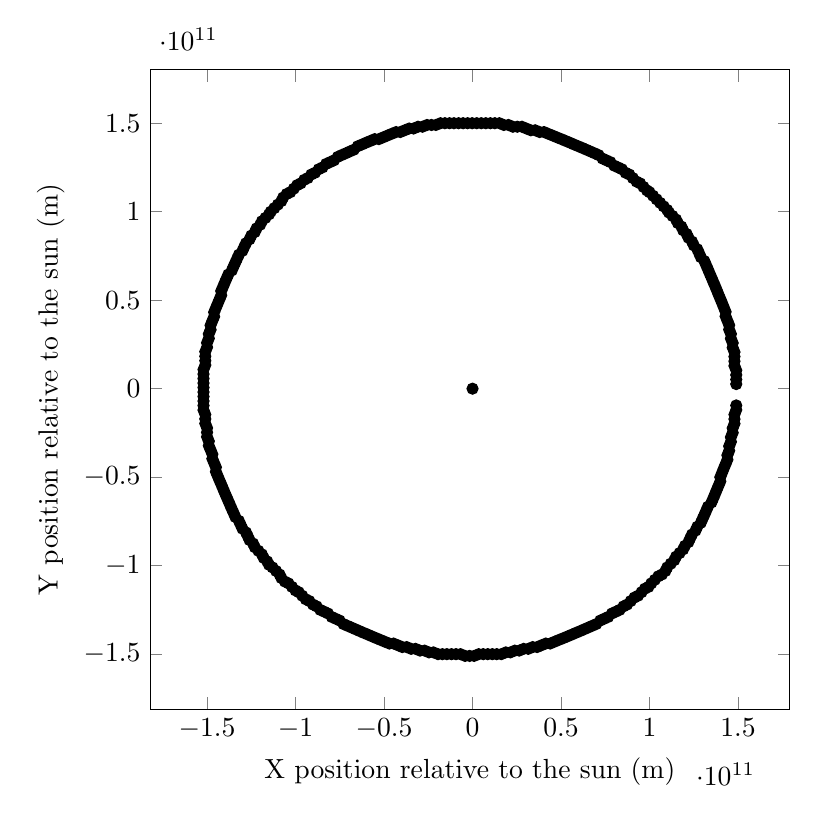
\begin{tikzpicture}
			\begin{axis}[%x
			width=0.8\textwidth,
			height=0.8\textwidth,
			xlabel={X position relative to the sun (m)},
			ylabel={Y position relative to the sun (m)},
			scatter/classes={%
				a={mark=o,draw=black}}]
			\addplot[scatter,only marks,%
			scatter src=explicit symbolic]%
			table[meta=x] {
				x	y
				0 0
				1.49E+11	2.59E+09
				1.49E+11	5.18E+09
				1.49E+11	7.77E+09
				1.49E+11	1.04E+10
				1.48E+11	1.29E+10
				1.48E+11	1.55E+10
				1.48E+11	1.81E+10
				1.48E+11	2.07E+10
				1.47E+11	2.32E+10
				1.47E+11	2.58E+10
				1.46E+11	2.83E+10
				1.46E+11	3.09E+10
				1.45E+11	3.34E+10
				1.45E+11	3.59E+10
				1.44E+11	3.84E+10
				1.43E+11	4.09E+10
				1.43E+11	4.34E+10
				1.42E+11	4.59E+10
				1.41E+11	4.84E+10
				1.40E+11	5.08E+10
				1.39E+11	5.32E+10
				1.38E+11	5.57E+10
				1.37E+11	5.81E+10
				1.36E+11	6.04E+10
				1.35E+11	6.28E+10
				1.34E+11	6.51E+10
				1.33E+11	6.75E+10
				1.32E+11	6.98E+10
				1.31E+11	7.21E+10
				1.29E+11	7.43E+10
				1.28E+11	7.66E+10
				1.27E+11	7.88E+10
				1.25E+11	8.10E+10
				1.24E+11	8.31E+10
				1.22E+11	8.53E+10
				1.21E+11	8.74E+10
				1.19E+11	8.95E+10
				1.18E+11	9.16E+10
				1.16E+11	9.36E+10
				1.15E+11	9.56E+10
				1.13E+11	9.76E+10
				1.11E+11	9.95E+10
				1.10E+11	1.01E+11
				1.08E+11	1.03E+11
				1.06E+11	1.05E+11
				1.04E+11	1.07E+11
				1.02E+11	1.09E+11
				1.00E+11	1.11E+11
				9.86E+10	1.12E+11
				9.66E+10	1.14E+11
				9.47E+10	1.16E+11
				9.27E+10	1.17E+11
				9.06E+10	1.19E+11
				8.86E+10	1.21E+11
				8.65E+10	1.22E+11
				8.44E+10	1.24E+11
				8.23E+10	1.25E+11
				8.01E+10	1.26E+11
				7.79E+10	1.28E+11
				7.57E+10	1.29E+11
				7.35E+10	1.30E+11
				7.12E+10	1.32E+11
				6.90E+10	1.33E+11
				6.67E+10	1.34E+11
				6.44E+10	1.35E+11
				6.21E+10	1.36E+11
				5.97E+10	1.37E+11
				5.73E+10	1.38E+11
				5.50E+10	1.39E+11
				5.26E+10	1.40E+11
				5.02E+10	1.41E+11
				4.77E+10	1.42E+11
				4.53E+10	1.43E+11
				4.28E+10	1.44E+11
				4.04E+10	1.45E+11
				3.79E+10	1.45E+11
				3.54E+10	1.46E+11
				3.29E+10	1.46E+11
				3.04E+10	1.47E+11
				2.79E+10	1.48E+11
				2.53E+10	1.48E+11
				2.28E+10	1.48E+11
				2.03E+10	1.49E+11
				1.77E+10	1.49E+11
				1.52E+10	1.50E+11
				1.26E+10	1.50E+11
				1.01E+10	1.50E+11
				7.50E+09	1.50E+11
				4.94E+09	1.50E+11
				2.37E+09	1.50E+11
				-1.96E+08	1.50E+11
				-2.76E+09	1.50E+11
				-5.33E+09	1.50E+11
				-7.89E+09	1.50E+11
				-1.05E+10	1.50E+11
				-1.30E+10	1.50E+11
				-1.56E+10	1.50E+11
				-1.81E+10	1.50E+11
				-2.07E+10	1.49E+11
				-2.32E+10	1.49E+11
				-2.57E+10	1.49E+11
				-2.83E+10	1.48E+11
				-3.08E+10	1.48E+11
				-3.33E+10	1.47E+11
				-3.58E+10	1.47E+11
				-3.83E+10	1.46E+11
				-4.08E+10	1.45E+11
				-4.32E+10	1.45E+11
				-4.57E+10	1.44E+11
				-4.81E+10	1.43E+11
				-5.05E+10	1.42E+11
				-5.29E+10	1.41E+11
				-5.53E+10	1.41E+11
				-5.77E+10	1.40E+11
				-6.01E+10	1.39E+11
				-6.24E+10	1.38E+11
				-6.48E+10	1.37E+11
				-6.71E+10	1.35E+11
				-6.94E+10	1.34E+11
				-7.16E+10	1.33E+11
				-7.39E+10	1.32E+11
				-7.61E+10	1.31E+11
				-7.83E+10	1.29E+11
				-8.05E+10	1.28E+11
				-8.27E+10	1.27E+11
				-8.48E+10	1.25E+11
				-8.69E+10	1.24E+11
				-8.90E+10	1.22E+11
				-9.11E+10	1.21E+11
				-9.31E+10	1.19E+11
				-9.51E+10	1.18E+11
				-9.71E+10	1.16E+11
				-9.91E+10	1.15E+11
				-1.01E+11	1.13E+11
				-1.03E+11	1.11E+11
				-1.05E+11	1.10E+11
				-1.07E+11	1.08E+11
				-1.08E+11	1.06E+11
				-1.10E+11	1.04E+11
				-1.12E+11	1.02E+11
				-1.14E+11	1.00E+11
				-1.15E+11	9.85E+10
				-1.17E+11	9.65E+10
				-1.19E+11 9.46E+10
				-1.20E+11 9.26E+10
				-1.22E+11 9.06E+10
				-1.23E+11 8.85E+10
				-1.25E+11 8.65E+10
				-1.26E+11 8.44E+10
				-1.28E+11 8.22E+10
				-1.29E+11 8.01E+10
				-1.30E+11 7.79E+10
				-1.32E+11 7.57E+10
				-1.33E+11 7.35E+10
				-1.34E+11 7.13E+10
				-1.35E+11 6.91E+10
				-1.36E+11 6.68E+10
				-1.38E+11 6.45E+10
				-1.39E+11 6.22E+10
				-1.40E+11 5.99E+10
				-1.41E+11 5.75E+10
				-1.42E+11 5.52E+10
				-1.42E+11 5.28E+10
				-1.43E+11 5.04E+10
				-1.44E+11 4.80E+10
				-1.45E+11 4.56E+10
				-1.46E+11 4.32E+10
				-1.46E+11 4.07E+10
				-1.47E+11 3.83E+10
				-1.48E+11 3.58E+10
				-1.48E+11 3.33E+10
				-1.49E+11 3.09E+10
				-1.49E+11 2.84E+10
				-1.50E+11 2.59E+10
				-1.50E+11 2.34E+10
				-1.51E+11 2.09E+10
				-1.51E+11 1.83E+10
				-1.51E+11 1.58E+10
				-1.51E+11 1.33E+10
				-1.52E+11 1.08E+10
				-1.52E+11 8.22E+09
				-1.52E+11 5.69E+09
				-1.52E+11 3.15E+09
				-1.52E+11 6.10E+08
				-1.52E+11 -1.93E+09
				-1.52E+11 -4.47E+09
				-1.52E+11 -7.01E+09
				-1.52E+11 -9.54E+09
				-1.52E+11 -1.21E+10
				-1.51E+11 -1.46E+10
				-1.51E+11 -1.71E+10
				-1.51E+11 -1.97E+10
				-1.50E+11 -2.22E+10
				-1.50E+11 -2.47E+10
				-1.50E+11 -2.72E+10
				-1.49E+11 -2.97E+10
				-1.49E+11 -3.22E+10
				-1.48E+11 -3.46E+10
				-1.47E+11 -3.71E+10
				-1.47E+11 -3.96E+10
				-1.46E+11 -4.20E+10
				-1.45E+11 -4.44E+10
				-1.45E+11 -4.69E+10
				-1.44E+11 -4.93E+10
				-1.43E+11 -5.17E+10
				-1.42E+11 -5.40E+10
				-1.41E+11 -5.64E+10
				-1.40E+11 -5.88E+10
				-1.39E+11 -6.11E+10
				-1.38E+11 -6.34E+10
				-1.37E+11 -6.57E+10
				-1.36E+11 -6.80E+10
				-1.35E+11 -7.02E+10
				-1.34E+11 -7.25E+10
				-1.32E+11 -7.47E+10
				-1.31E+11 -7.69E+10
				-1.30E+11 -7.91E+10
				-1.28E+11 -8.12E+10
				-1.27E+11 -8.33E+10
				-1.26E+11 -8.55E+10
				-1.24E+11 -8.75E+10
				-1.23E+11 -8.96E+10
				-1.21E+11 -9.16E+10
				-1.19E+11 -9.36E+10
				-1.18E+11 -9.56E+10
				-1.16E+11 -9.76E+10
				-1.15E+11 -9.95E+10
				-1.13E+11 -1.01E+11
				-1.11E+11 -1.03E+11
				-1.09E+11 -1.05E+11
				-1.08E+11 -1.07E+11
				-1.06E+11 -1.09E+11
				-1.04E+11 -1.10E+11
				-1.02E+11 -1.12E+11
				-1.00E+11 -1.14E+11
				-9.82E+10 -1.15E+11
				-9.62E+10 -1.17E+11
				-9.42E+10 -1.19E+11
				-9.22E+10 -1.20E+11
				-9.01E+10 -1.22E+11
				-8.81E+10 -1.23E+11
				-8.60E+10 -1.25E+11
				-8.38E+10 -1.26E+11
				-8.17E+10 -1.27E+11
				-7.95E+10 -1.29E+11
				-7.73E+10 -1.30E+11
				-7.51E+10 -1.31E+11
				-7.29E+10 -1.33E+11
				-7.06E+10 -1.34E+11
				-6.83E+10 -1.35E+11
				-6.60E+10 -1.36E+11
				-6.37E+10 -1.37E+11
				-6.14E+10 -1.38E+11
				-5.90E+10 -1.39E+11
				-5.67E+10 -1.40E+11
				-5.43E+10 -1.41E+11
				-5.19E+10 -1.42E+11
				-4.95E+10 -1.43E+11
				-4.70E+10 -1.44E+11
				-4.46E+10 -1.44E+11
				-4.21E+10 -1.45E+11
				-3.97E+10 -1.46E+11
				-3.72E+10 -1.46E+11
				-3.47E+10 -1.47E+11
				-3.22E+10 -1.47E+11
				-2.97E+10 -1.48E+11
				-2.71E+10 -1.48E+11
				-2.46E+10 -1.49E+11
				-2.21E+10 -1.49E+11
				-1.95E+10 -1.50E+11
				-1.70E+10 -1.50E+11
				-1.45E+10 -1.50E+11
				-1.19E+10 -1.50E+11
				-9.34E+09 -1.50E+11
				-6.78E+09 -1.50E+11
				-4.21E+09 -1.51E+11
				-1.65E+09 -1.51E+11
				9.16E+08 -1.51E+11
				3.48E+09 -1.50E+11
				6.04E+09 -1.50E+11
				8.61E+09 -1.50E+11
				1.12E+10 -1.50E+11
				1.37E+10 -1.50E+11
				1.63E+10 -1.50E+11
				1.88E+10 -1.49E+11
				2.14E+10 -1.49E+11
				2.39E+10 -1.48E+11
				2.64E+10 -1.48E+11
				2.89E+10 -1.47E+11
				3.15E+10 -1.47E+11
				3.40E+10 -1.46E+11
				3.65E+10 -1.46E+11
				3.89E+10 -1.45E+11
				4.14E+10 -1.44E+11
				4.39E+10 -1.44E+11
				4.63E+10 -1.43E+11
				4.87E+10 -1.42E+11
				5.12E+10 -1.41E+11
				5.36E+10 -1.40E+11
				5.60E+10 -1.39E+11
				5.83E+10 -1.38E+11
				6.07E+10 -1.37E+11
				6.30E+10 -1.36E+11
				6.53E+10 -1.35E+11
				6.76E+10 -1.34E+11
				6.99E+10 -1.33E+11
				7.22E+10 -1.31E+11
				7.44E+10 -1.30E+11
				7.66E+10 -1.29E+11
				7.88E+10 -1.27E+11
				8.10E+10 -1.26E+11
				8.31E+10 -1.25E+11
				8.53E+10 -1.23E+11
				8.73E+10 -1.22E+11
				8.94E+10 -1.20E+11
				9.15E+10 -1.18E+11
				9.35E+10 -1.17E+11
				9.55E+10 -1.15E+11
				9.74E+10 -1.13E+11
				9.94E+10 -1.12E+11
				1.01E+11 -1.10E+11
				1.03E+11 -1.08E+11
				1.05E+11 -1.06E+11
				1.07E+11 -1.05E+11
				1.09E+11 -1.03E+11
				1.10E+11 -1.01E+11
				1.12E+11 -9.89E+10
				1.14E+11 -9.69E+10
				1.15E+11 -9.49E+10
				1.17E+11 -9.29E+10
				1.19E+11 -9.08E+10
				1.20E+11 -8.88E+10
				1.22E+11 -8.67E+10
				1.23E+11 -8.45E+10
				1.24E+11 -8.24E+10
				1.26E+11 -8.02E+10
				1.27E+11 -7.80E+10
				1.29E+11 -7.58E+10
				1.30E+11 -7.35E+10
				1.31E+11 -7.13E+10
				1.32E+11 -6.90E+10
				1.33E+11 -6.67E+10
				1.35E+11 -6.43E+10
				1.36E+11 -6.20E+10
				1.37E+11 -5.96E+10
				1.38E+11 -5.72E+10
				1.39E+11 -5.48E+10
				1.40E+11 -5.24E+10
				1.40E+11 -5.00E+10
				1.41E+11 -4.75E+10
				1.42E+11 -4.50E+10
				1.43E+11 -4.26E+10
				1.44E+11 -4.01E+10
				1.44E+11 -3.76E+10
				1.45E+11 -3.51E+10
				1.45E+11 -3.25E+10
				1.46E+11 -3.00E+10
				1.46E+11 -2.74E+10
				1.47E+11 -2.49E+10
				1.47E+11 -2.23E+10
				1.48E+11 -1.98E+10
				1.48E+11 -1.72E+10
				1.48E+11 -1.46E+10
				1.49E+11 -1.20E+10
				1.49E+11 -9.46E+09
				
			};
			\end{axis}
		\end{tikzpicture}
		\caption{Simulated orbit of earth over 365 days}
		\label{fig:graphEarth}
	\end{figure}
	
	As you can see in Figure 13, the simulation correctly simulates the orbital period of the earth to be about 365 days. This is very close to the actual period of 365.256 days. The differences are probably down to the precision of the data I used to set up the simulation and the nature of that data being averages.
	
	I also simulated the orbit of the moon around the earth. As you can see (Figure 15) it correctly simulates the orbital period to be just over 27 days (the true value is 27.323).
	

	The data used are listed in the table below
	
	\begin{figure}[h]
		\centering
		\begin{tabular}{ | l | c | c | c |}
			\hline
			\textbf{Particle} & \textbf{Mass (kg)} & \textbf{Distance (m)} & \textbf{Speed (m/s)} \\ \hline
			Earth & $5.9724\times10^{24}$ & $149\times10^9$ (from sun) & $30\times10^3$ (relative to sun) \\ \hline
			Sun & $1.989\times10^{30}$ & -- & -- \\ \hline
			Moon & $7.346\times10^{22}$ & $385\times10^{6}$  & $1022$ (relative to earth) \\	\hline
		\end{tabular}
		\caption{Data used in simulations of real-world orbits}
		\label{table:data}
	\end{figure}
		
	These examples show that gravity is simulated correctly and with an acceptable degree of accuracy.
	
	\begin{figure}[p]
			\begin{subfigure}{0.48\textwidth}
				\begin{tikzpicture}
				\begin{axis}[%x
				width=0.9\textwidth,
				height=0.9\textwidth,
				xlabel={X position (m)},
				ylabel={Y position (m)},
				ymin=-4E+08,
				scatter/classes={%
					a={mark=o,draw=black}}]
				\addplot[scatter,only marks,%
				scatter src=explicit symbolic]%
				table[meta=day] {
					x y day
					0 0 0
					3.75E+08	8.39E+07	1
					3.46E+08	1.67E+08	2
					2.99E+08	2.42E+08	3
					2.36E+08	3.04E+08	4
					1.61E+08	3.50E+08	5
					7.80E+07	3.78E+08	6
					-9416243.201	3.87E+08	7
					-9.63E+07	3.75E+08	8
					-1.78E+08	3.45E+08	9
					-2.51E+08	2.97E+08	10
					-3.12E+08	2.34E+08	11
					-3.57E+08	1.60E+08	12
					-3.84E+08	7.76E+07	13
					-3.92E+08	-8622263.529	14
					-3.81E+08	-9.44E+07	15				
				};	
				\end{axis}
				\end{tikzpicture}
				\caption{Simulated orbit of moon over 15 days}
				\label{fig:graphMoon1}
			\end{subfigure}
			\begin{subfigure}{0.48\textwidth}
				\begin{tikzpicture}
				\begin{axis}[%x
				width=0.9\textwidth,
				height=0.9\textwidth,
				xlabel={X position (m)},
				ylabel={Y position (m)},
				scatter/classes={%
					a={mark=o,draw=black}}]
				\addplot[scatter,only marks,%
				scatter src=explicit symbolic]%
				table[meta=day] {
					x y day
					0 0 0
					3.75E+08	8.39E+07	1
					3.46E+08	1.67E+08	2
					2.99E+08	2.42E+08	3
					2.36E+08	3.04E+08	4
					1.61E+08	3.50E+08	5
					7.80E+07	3.78E+08	6
					-9416243.201	3.87E+08	7
					-9.63E+07	3.75E+08	8
					-1.78E+08	3.45E+08	9
					-2.51E+08	2.97E+08	10
					-3.12E+08	2.34E+08	11
					-3.57E+08	1.60E+08	12
					-3.84E+08	7.76E+07	13
					-3.92E+08	-8622263.529	14
					-3.81E+08	-9.44E+07	15
					-3.51E+08	-1.76E+08	16
					-3.04E+08	-2.48E+08	17
					-2.42E+08	-3.09E+08	18
					-1.68E+08	-3.54E+08	19
					-8.59E+07	-3.81E+08	20
					502665.788	-3.90E+08	21
					8.69E+07	-3.80E+08	22
					1.69E+08	-3.50E+08	23
					2.42E+08	-3.03E+08	24
					3.03E+08	-2.40E+08	25
					3.49E+08	-1.65E+08	26
					3.77E+08	-8.14E+07	27	
				};	
				\end{axis}
				\end{tikzpicture}
				\caption{Simulated orbit of moon over 27 days}
				\label{fig:graphMoon2}
			\end{subfigure}
			\begin{subfigure}{0.9\textwidth}
				\centering
				\begin{tikzpicture}
				\begin{axis}[%x
				width=\textwidth,
				height=\textwidth,
				xlabel={X position - relative to sun at (0,0) (m)},
				ylabel={Y position - relative to sun at (0,0) (m)},
				scatter/classes={%
					a={mark=o,draw=black}}]
				\addplot[scatter,only marks,%
				scatter src=explicit symbolic, mark size=1.4]%
				table[meta=day] {
					x y day
					1.48978731E+11	2.48389460E+09	1.00000000E+00
					1.48913074E+11	5.07509887E+09	2.00000000E+00
					1.48803030E+11	7.66488998E+09	3.00000000E+00
					1.48648604E+11	1.02525400E+10	4.00000000E+00
					1.48449803E+11	1.28373137E+10	5.00000000E+00
					1.48206640E+11	1.54184667E+10	6.00000000E+00
					1.47919137E+11	1.79952449E+10	7.00000000E+00
					1.47587326E+11	2.05668832E+10	8.00000000E+00
					1.47211251E+11	2.31326054E+10	9.00000000E+00
					1.46790974E+11	2.56916244E+10	1.00000000E+01
					1.46326574E+11	2.82431420E+10	1.10000000E+01
					1.45818152E+11	3.07863507E+10	1.20000000E+01
					1.45265833E+11	3.33204354E+10	1.30000000E+01
					1.44669772E+11	3.58445772E+10	1.40000000E+01
					1.44030153E+11	3.83579579E+10	1.50000000E+01
					1.43347188E+11	4.08597649E+10	1.60000000E+01
					1.42621120E+11	4.33491965E+10	1.70000000E+01
					1.41852214E+11	4.58254653E+10	1.80000000E+01
					1.41040759E+11	4.82878012E+10	1.90000000E+01
					1.40187060E+11	5.07354520E+10	2.00000000E+01
					1.39291436E+11	5.31676836E+10	2.10000000E+01
					1.38354216E+11	5.55837793E+10	2.20000000E+01
					1.37375740E+11	5.79830386E+10	2.30000000E+01
					1.36356353E+11	6.03647766E+10	2.40000000E+01
					1.35296406E+11	6.27283229E+10	2.50000000E+01
					1.34196254E+11	6.50730202E+10	2.60000000E+01
					1.33056254E+11	6.73982235E+10	2.70000000E+01
					1.31876763E+11	6.97032977E+10	2.80000000E+01
					1.30658139E+11	7.19876152E+10	2.90000000E+01
					1.29400737E+11	7.42505537E+10	3.00000000E+01					
				};\addplot[scatter, mark size=1, only marks,scatter src=explicit symbolic, color=red] table[meta=day] {
				x y day
				1.49354135E+11	2.56783155E+09	3.10000000E+01
				1.49259330E+11	5.24220943E+09	3.20000000E+01
				1.49102079E+11	7.90631710E+09	3.30000000E+01
				1.48884836E+11	1.05554729E+10	3.40000000E+01
				1.48610880E+11	1.31856510E+10	3.50000000E+01
				1.48284140E+11	1.57936345E+10	3.60000000E+01
				1.47909009E+11	1.83771256E+10	3.70000000E+01
				1.47490158E+11	2.09348218E+10	3.80000000E+01
				1.47032332E+11	2.34664671E+10	3.90000000E+01
				1.46540128E+11	2.59728771E+10	4.00000000E+01
				1.46017762E+11	2.84559267E+10	4.10000000E+01
				1.45468789E+11	3.09184772E+10	4.20000000E+01
				1.44895843E+11	3.33642164E+10	4.30000000E+01
				1.44300394E+11	3.57973973E+10	4.40000000E+01
				1.43682607E+11	3.82224872E+10	4.50000000E+01
				1.43041323E+11	4.06437720E+10	4.60000000E+01
				1.42374188E+11	4.30649777E+10	4.70000000E+01
				1.41677896E+11	4.54889740E+10	4.80000000E+01
				1.40948495E+11	4.79175930E+10	4.90000000E+01
				1.40181700E+11	5.03515641E+10	5.00000000E+01
				1.39373165E+11	5.27905378E+10	5.10000000E+01
				1.38518706E+11	5.52331608E+10	5.20000000E+01
				1.37614469E+11	5.76771720E+10	5.30000000E+01
				1.36657072E+11	6.01195005E+10	5.40000000E+01
				1.35643730E+11	6.25563646E+10	5.50000000E+01
				1.34572374E+11	6.49833793E+10	5.60000000E+01
				1.33441781E+11	6.73956876E+10	5.70000000E+01
				1.32251677E+11	6.97881305E+10	5.80000000E+01
				1.31002828E+11	7.21554601E+10	5.90000000E+01
				1.29697059E+11	7.44925890E+10	6.00000000E+01
			};
			\end{axis}
			\end{tikzpicture}
			\caption{Simulated orbit of moon (red) and earth (black)}
			\label{fig:graphMoon2}
		\end{subfigure}
		\caption{Simulated orbit of the moon and earth}
		\label{fig:graphMoon}
	\end{figure}
	
	\subsection{Collisions}
	The collisions I implemented on the other hand were less successful. I was unable to find a simple solution to elastic collisions in two dimensions. To try and overcome this I used the method I discussed in section 4. This gives what seem like plausible results when watched in the simulation and it successfully conserves momentum.
	
	The problem is that the collisions do not preserve kinetic energy, infact they create it. If I had more time I would spend longer and derive equations myself. As this project was meant to be about gravity this is not too much of a problem. Figures 16 and 17 show some tests of the collisions
	
	\begin{figure}[p]
		\centering
		\begin{subfigure}{0.49\textwidth}
			\centering
			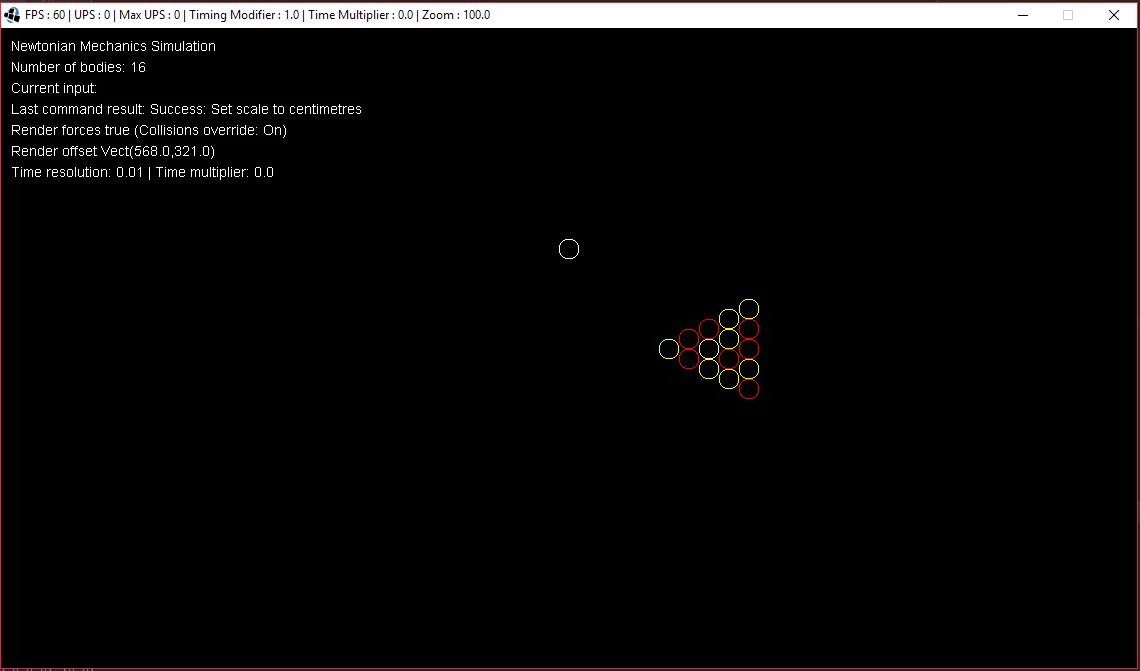
\includegraphics[width=\textwidth]{pool1}
			\caption{Pool simulation before any collisions}
			\label{fig:colEval1Sub1}
		\end{subfigure}
		\begin{subfigure}{0.49\textwidth}
			\centering
			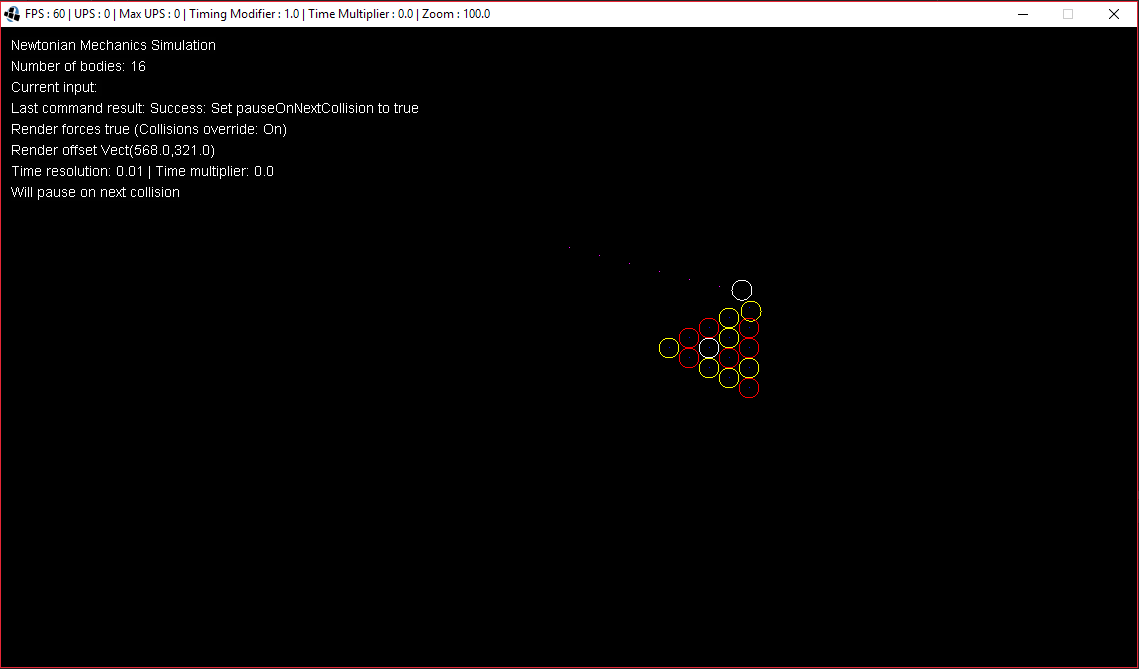
\includegraphics[width=\textwidth]{pool2}
			\caption{First impact of white ball on the triangle} 
			\label{fig:colEval1Sub2}
		\end{subfigure}	
		\begin{subfigure}{0.49\textwidth}
			\centering
			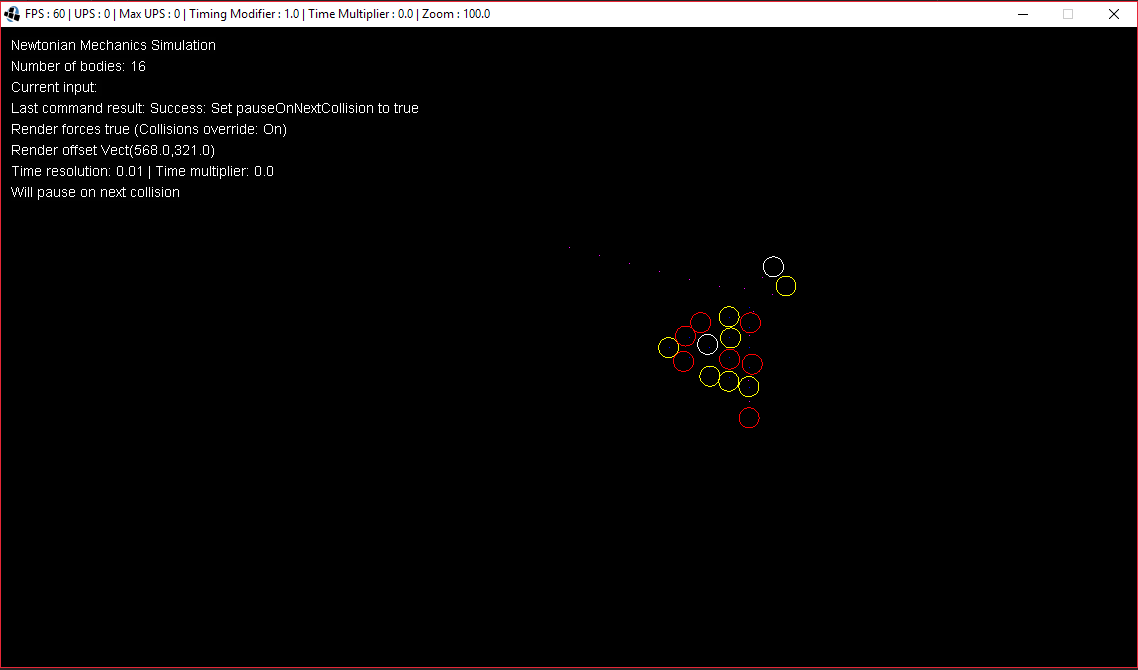
\includegraphics[width=\textwidth]{pool3}
			\caption{More collisions lead the triangle to split up} 
			\label{fig:colEval1Sub3}
		\end{subfigure}	
		\begin{subfigure}{0.49\textwidth}
			\centering
			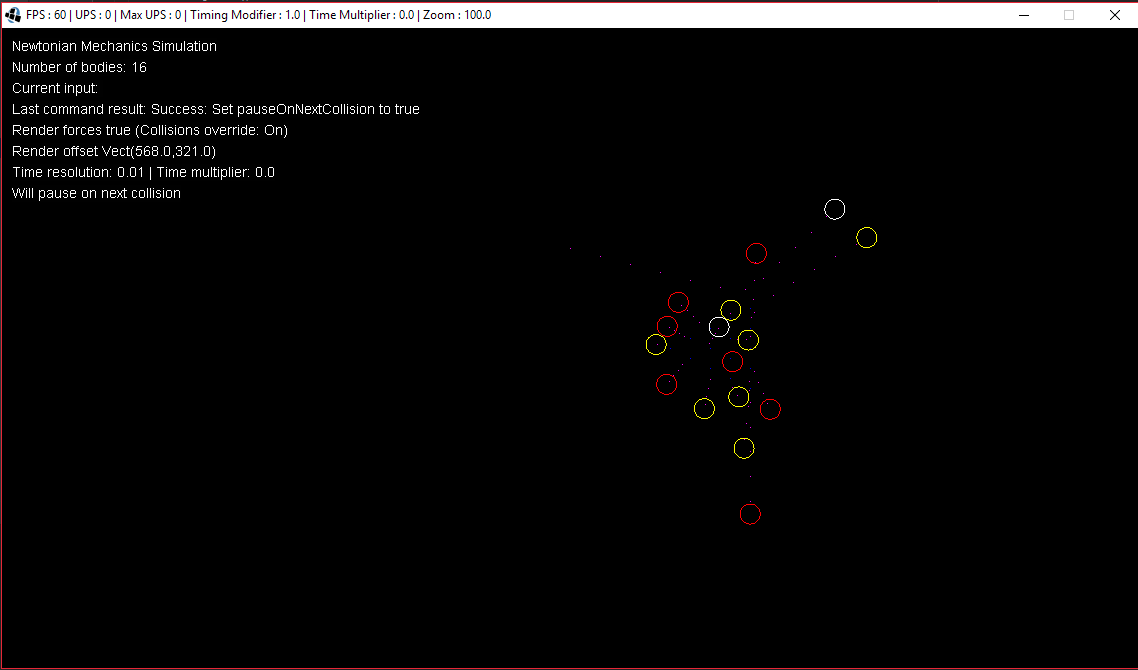
\includegraphics[width=\textwidth]{pool4}
			\caption{Result of the break} 
			\label{fig:colEval1Sub4}
		\end{subfigure}	
		\caption{A pool-style break with 1kg balls, with 10cm radii. The white has an initial velocity of 6.17m/s}
		\label{fig:colEval1}
	\end{figure}
	
	\begin{figure}[p]
		\centering
		\begin{subfigure}{0.49\textwidth}
			\centering
			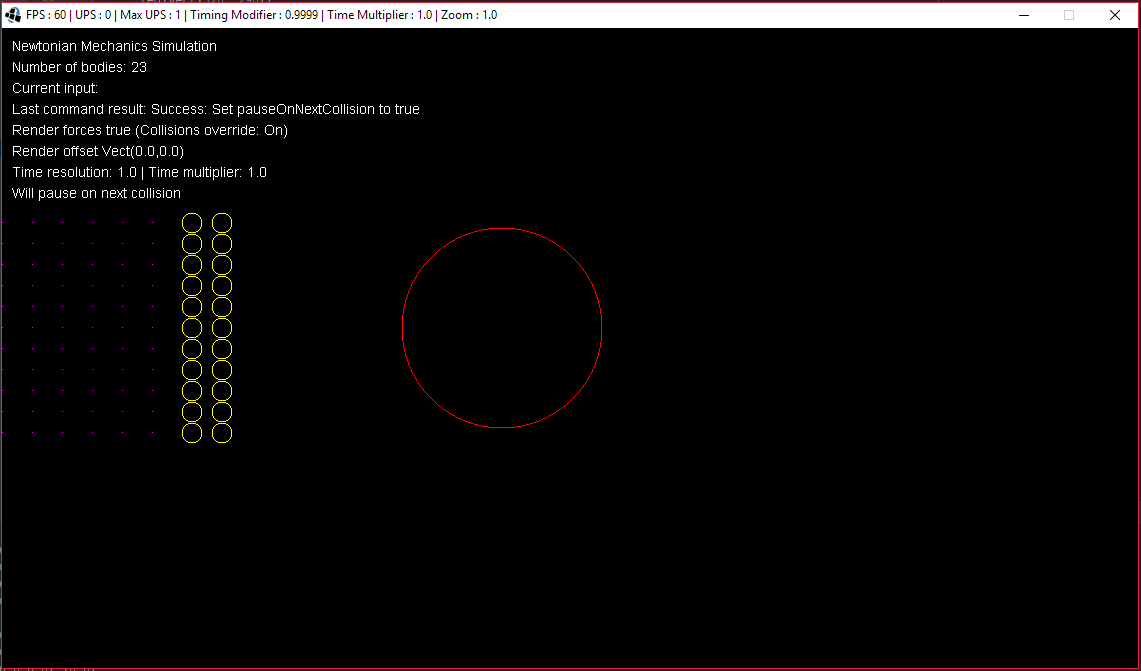
\includegraphics[width=\textwidth]{bigCol1}
			\caption{The set-up for the simulation. The yellow balls are travelling right.}
			\label{fig:colEval2Sub1}
		\end{subfigure}
		\begin{subfigure}{0.49\textwidth}
			\centering
			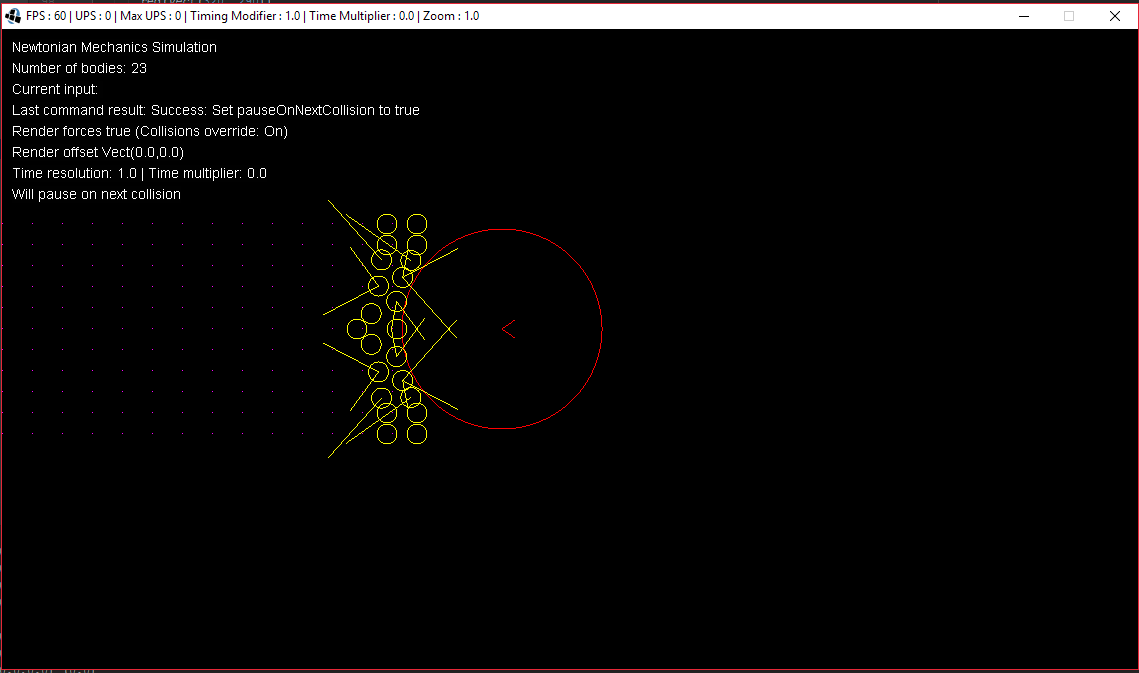
\includegraphics[width=\textwidth]{bigCol2}
			\caption{Result of the simulation with forces drawn to show the collisions} 
			\label{fig:colEval2Sub2}
		\end{subfigure}	
		\caption{A test simulation that demonstrates the conservation of momentum. Momentum before and after is $1100kgm/s$}
		\label{fig:colEval2}
	\end{figure}

\end{document}
